\documentclass[12pt,letterpaper,noanswers]{exam}
\usepackage[usenames,dvipsnames,svgnames,table]{xcolor}
\usepackage[margin=0.9in]{geometry}
\renewcommand{\familydefault}{\sfdefault}
\usepackage{multicol}
\usepackage{wrapfig}
\pagestyle{head}
\definecolor{c03}{HTML}{FFDDDD}
\header{AM 22b Class 24}{}{Mar 26: A circulation theorem, p.\thepage}
\runningheadrule
\headrule
\usepackage{graphicx} % more modern
\usepackage{amsmath} 
\usepackage{amssymb} 
\usepackage{hyperref}
\usepackage{tcolorbox}
\usepackage[utf8]{inputenc}
\usepackage{diagbox}
\usepackage{graphicx} 
\usepackage{enumitem}
\usepackage{tikz}
\tikzstyle{startstop} = [rectangle, rounded corners, minimum width=3cm, minimum height=1cm,text centered, draw=black]

\tikzstyle{process} = [rectangle, minimum width=3cm, minimum height=1cm, text centered, draw=black, fill=gray!20]
\tikzstyle{decision} = [ellipse, minimum width=3cm, minimum height=0.5cm, text centered, draw=black, fill=white!30]
\tikzstyle{arrow} = [thick,->,>=stealth]
\usetikzlibrary{shapes.geometric, arrows}
\pagenumbering{arabic}

\usepackage[numbered,autolinebreaks,useliterate]{mcode}

\newcommand{\mb}[1]{\underline{#1}}

\begin{document}
 \pdfpageheight 11in 
  \pdfpagewidth 8.5in


\begin{itemize}
% \item There is a pre-class assignment (20 minutes of videos + a few WeBWorK exercises) due at 10am this Monday.  It is available on Canvas.
\itemsep0em
    \item Problem set 07 is due on Thursday April 1st.
    \item Our next quiz will be Friday April 2nd.
    \item There will be a pre-class assignment for Monday March 29th.
   \item The next skill check is for C22, 23, 24 and is on Monday, March 29th.
\end{itemize}

\hrule
\vspace{0.2cm}

% partial derivatives, gradient
% local linearity, differential, directional deriv
% 2nd order partials + equations with partials

\noindent\textbf{Big picture}

When a vector field is a gradient field, the fundamental theorem of calculus for line integrals provides an alternative method of calculating a line integral.  Today's class focuses on a theorem that can be used to compute circulation when a vector field is not a gradient field.

\vspace{0.2cm}
\hrule
\vspace{0.2cm}

\noindent\textbf{Skill Check C24 Practice}.  
 Find the scalar curl for $\mb F = \langle y, xy \rangle$.  Then identify whether $\mb F$ is an irrotational vector field, or not.

\vspace{0.2cm}
\hrule
\vspace{0.2cm}

\noindent\textbf{Skill Check C24 Practice Solution}.  
$Q = xy$, $P = y$.  $Q_x = y$.  $P_y = 1$.  $Q_x - P_y = y-1$.
The scalar curl is $y-1$, which is sometimes nonzero, so $\mb F$ is not irrotational.  

\vspace{0.2cm}
\hrule
\vspace{0.2cm}

\noindent\textbf{Teams}
% Dabao, James, Taylor, Akhila, Jonny

\begin{multicols}{2}

1.  student names
\end{multicols}

\vspace{0.2cm}
\hrule
\vspace{0.2cm}

\vspace{0.2cm}
\hrule
\vspace{0.2cm}


\noindent\textbf{Path independent vector fields are equivalent to circulation-free vector fields} \S 18.3
\begin{tcolorbox}
\begin{itemize}
\itemsep0em
    \item A vector field is called \textbf{circulation free} when $\displaystyle\oint_C \mb F\cdot d\mb r = 0$ for all curves $C$ in the domain of $\mb F$.
    \item The term circulation-free is used in engineering applications, particularly to describe velocity vectors fields in fluids.
\end{itemize}
\end{tcolorbox} 



\noindent\textbf{Example (circulation free)}.  Let $\mb F$ be a path independent vector field.  Let $C$ be a simple closed curve with negative orientation (clockwise) with $P$ and $Q$ two distinct points on the curve.  Let $C_1$ and $C_2$ be paths from $P$ to $Q$ with orientations as shown in the figure below.

\begin{multicols}{2}
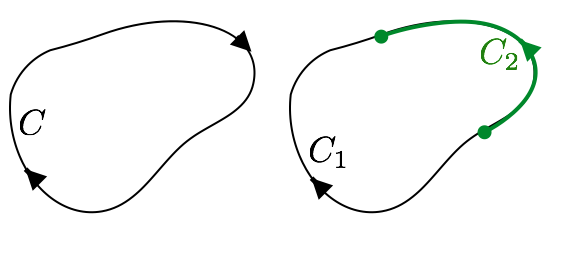
\includegraphics[width=2.5in]{img/C27p2.png}

Rewrite $\displaystyle\oint_C \mb F\cdot d\mb r$  using $C_1$ and $C_2$. 
\end{multicols}
\vspace{0.5in}




% \vfill

% \noindent\textbf{Path independent field = gradient field}.  Gradient vector fields are always path-independent vector fields.  Are path-independent vector fields always gradient fields? (Yes).

% Given a path-independent vector field, choose a point $P_0$ to be the \emph{ground}, with the potential $f(P_0) = 0$.  Let $f(Q) = \int_C \mb F\cdot d\mb r$ where $C$ is a path from $P_0$ to $Q$ (and $f(Q)$ is the work done by the vector field in moving an object from $P_0$ to $Q$).

% If $\mb\nabla f = \mb F$ then $\mb F$ is a gradient field.  The course text has a careful argument in section 18.3 (see text for details) showing that $\mb\nabla f = \mb F$, so path-independent vector fields are always gradient fields.

% \vfill

\vspace{0.2cm}
\hrule
\vspace{0.2cm}


\noindent\textbf{Constructing a potential function}
\begin{tcolorbox}
\begin{itemize}
    \item Given a vector field, $\nabla f$, we can construct a potential function, $f$.
    \item Given $\nabla f= \langle P,Q,R\rangle$, we have $P =f_x, Q=f_y, R=f_z$.  
\begin{enumerate}
    \item Let $f = \int P dx + g(y,z)$ where $g(y,z)$ is an unknown function of $y$ and $z$.  
    \item We have $f_y = \frac{\partial}{\partial y}\int P dx + g_y(y,z)$.  Assume $f_y = Q$ and rearrange to find $g_y(y,z)$.
    \item We now have $f = \int P dx + \int g_y dy + h(z)$.
    \item We have $f_z = \frac{\partial}{\partial z}\left(\int P dx +\int g_y dy \right)+ h_z$. Assume $f_z = R$ and rearrange to find $h_z$.
    \item Let $f = \int P dx + \int g_y dy + \int h_z dz$.  This is a possible potential function for the vector field.
\end{enumerate} 
\end{itemize}
\end{tcolorbox}
\noindent\textbf{Example (2d)}

Find $f$ if $\nabla f = \langle 2xy, x^2+y\rangle$.

\begin{enumerate}
    \item Let $f = \int 2xy dx + g(y) = x^2y + g(y)$.
    \item $f_y = x^2 + g_y = x^2+2y$, so $g_y = 2y$.
    \item $f = x^2y + \int 2ydy = x^2y + y^2$ works as a potential function.  $f=x^2y+y^2+3$ would work as well.
\end{enumerate}

\noindent\textbf{Example}
Calculate the line integral $\int_C \nabla f \cdot d\mb r$ exactly, where $\displaystyle\nabla f = \left\langle 2xe^{x^2+yz}, ze^{x^2+yz}, ye^{x^2+yz}\right\rangle$ and $C$ is a curve in the plane $z=0$ as shown below.

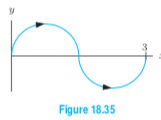
\includegraphics{img/C22p2.png}


\vfill

\noindent\textbf{Problem}.  Let $\mb r = x\mb i + y\mb j + z\mb k$ and $\mb a = a_1\mb i + a_2\mb j + a_3\mb k$.  Let $C$ be a path from the origin to the point with position vector $\mb r_0$.  Find $\int_C \nabla(\mb r\cdot \mb a)\cdot d\mb r$.  What is the maximum possible value of this line integral if $\Vert \mb r_0\Vert = 10?$
\vfill



\noindent\textbf{Question}.  Given a vector field $\mb F = \langle P, Q, R\rangle$, assume $\displaystyle\mb F = \left\langle \frac{\partial f}{\partial x}, \frac{\partial f}{\partial y}, \frac{\partial f}{\partial z}\right\rangle$.

Given this assumption, and assuming equality of mixed partials, provide relationships between $P_y, P_z, Q_x, Q_z, R_x, R_y$ that must be satisfied.


\eject
\vspace{0.2cm}
\hrule
\vspace{0.2cm}


\noindent\textbf{When is a vector field a gradient field?} \S 18.4

\begin{tcolorbox}
\begin{itemize}
\itemsep0em
    % \item Can you show the vector field isn't a gradient field?
    % \begin{itemize}
    %     \item Find a simple closed curve on which $\oint_C \mb F \cdot \mb T ds \neq 0$.  (Then the vector field is not circulation free, so is not a gradient field).
    %     \item Recall that $f_{xy} = f_{yx}$, $f_{yz} = f_{zy}$, $f_{zx} = f_{xz}$ (equality of mixed partials).  A gradient vector field is of the form $\nabla f = \langle f_x, f_y, f_z\rangle$.  Given a vector field $\mb F = \langle P,Q,R\rangle$, check whether equality of mixed partials is possible: $Q_x-P_y$, $R_y - Q_z$, $P_z - R_x$.  It any of these are nonzero it would not be possible for $\mb F$ to be a gradient field.
    % \end{itemize}
    \item $Q_x-P_y$ is called the scalar \textbf{curl}.
    \item $Q_x-P_y$, $R_y - Q_z$, $P_z - R_x$ are the three components of the vector \textbf{curl}.  \emph{We will wait to discuss vector curl - for now we'll work in 2D.}
    \item A vector field $\mb F = P\mb i +Q\mb j$ is called \textbf{irrotational} or \textbf{curl free} if $\displaystyle\frac{\partial Q}{\partial x}-\frac{\partial P}{\partial y}=0$
    \item A vector field $\mb F = P\mb i +Q\mb j +R\mb k$ is called \textbf{irrotational} or \textbf{curl free} if $\displaystyle\frac{\partial Q}{\partial x}-\frac{\partial P}{\partial y}=0,$ $\displaystyle\frac{\partial R}{\partial y} - \frac{\partial Q}{\partial z}=0,$ and $\displaystyle\frac{\partial P}{\partial z} - \frac{\partial R}{\partial x}=0.$
    \item A gradient vector field is irrotational (curl free).
    \item The term \textbf{irrotational} is used in fluid dynamics (engineering) to refer to fluids that do not have vorticity.
\end{itemize}
\end{tcolorbox}


\noindent\textbf{Example}.  Find the scalar curl for 
\begin{enumerate}
\itemsep3em
    \item $\mb F(x,y) = (x^2-y^2)\mb i - 2xy\mb j$.
    \item $\mb G(x,y) = -y\mb i + x \mb j$.
    \vspace{0.5in}
\end{enumerate}

Is $\mb F$ possibly a gradient vector field based on your scalar curl calculation?  Is $G$?
\emph{pollQ}

\vspace{1in}

\vspace{0.2cm}
\hrule
\vspace{0.2cm}
\noindent\textbf{What is scalar curl?} \S 18.4
\begin{tcolorbox}
\begin{itemize}
\itemsep0em
    \item Let $\mb F = \langle P,Q\rangle$.  The scalar curl, $\frac{\partial Q}{\partial x} - \frac{\partial P}{\partial y} \approx \frac{\Delta Q}{\Delta y} - \frac{\Delta P}{\Delta x}$.  The first term is the change in the length of the $\mb j$ component divided by a displacement in $x$.  The second term is the change in the length of the $\mb i$ component divided by a displacement in $y$.
\end{itemize}
\end{tcolorbox}

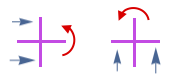
\includegraphics[height=1in]{img/C28p1-18.png}

\noindent\textbf{Question (scalar curl)}.  Identify the sign of the scalar curl for each of the vector fields below.

\hspace{-0.5in}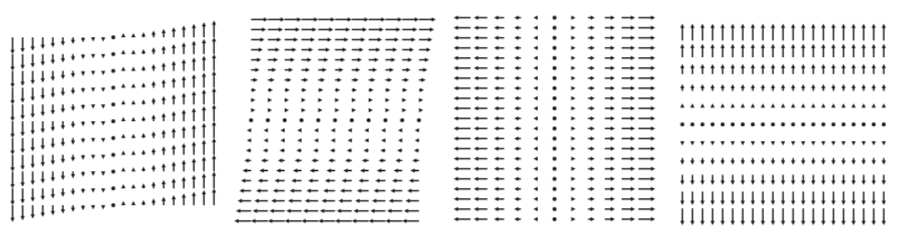
\includegraphics[width=\linewidth]{img/C24p2b-18.png}

\emph{pollQ}.
\vspace{1in}


\noindent\textbf{Sign of scalar curl for vector fields with $\mb i$ and $\mb j$ components}.  \S 18.4
\begin{tcolorbox}
For a vector field with $\mb F = P\mb i + Q\mb j$, think of the vector field as the sum of $\mb G = P\mb i$ and $\mb H = Q\mb j$ to identify the sign of the scalar curl.  If $Q_x$ and $-P_y$ have the same sign, then the sign of the scalar curl can be identified.  If they have different signs, their relative size will determine the sign of the scalar curl.
\end{tcolorbox}

\noindent\textbf{Example (sign of scalar curl)}.  If possible, determine the sign of the scalar curl for the vector field below.  On the left is shown $\mb F = M\mb i + N\mb j$.  On the right are shown $\mb G = M\mb i$ in blue and $\mb H = N\mb j$ in red.

\emph{pollQ}

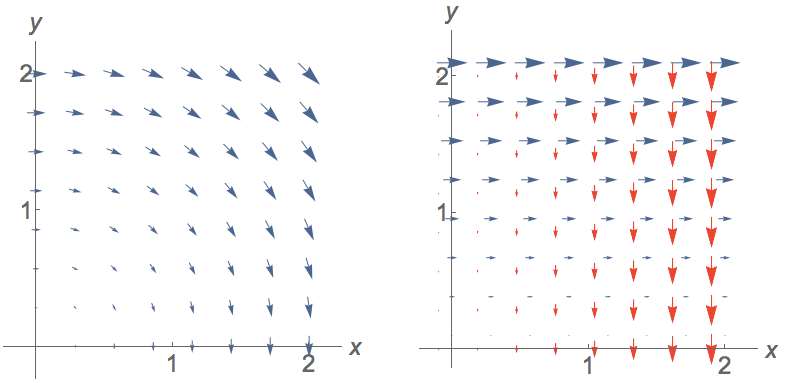
\includegraphics[width=5in]{img/C28p5.png}

\eject

\noindent\textbf{Examples (compute scalar curl)}. 
The vector fields below are
$\mb F_1 = \mb r$, $\mb F_{2} = \frac{\mb r}{\Vert \mb r\Vert}$.  $\mb F_{3} = x\mb j$.  $\mb F_{4} = y\mb i - x\mb j.$  Compute the scalar curl for each vector field.


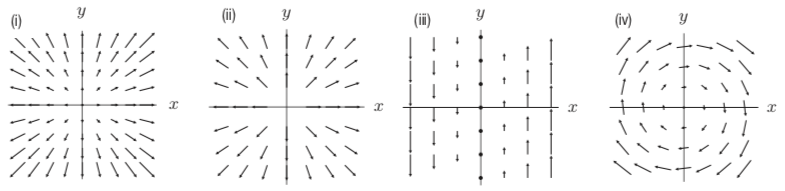
\includegraphics[width=\linewidth]{img/C23p1.png}
\vspace{1.5in}



\vspace{0.2cm}
\hrule
\vspace{0.2cm}

\noindent\textbf{Circulation integrals can be 'broken down' into smaller curves} \S 18.4
\begin{tcolorbox}
\begin{itemize}
\itemsep0em
\item $\int_C \mb F \cdot d\mb r = \int_{C_1} \mb F \cdot d\mb r + \int_{C_2} \mb F \cdot d\mb r$ where $C$ is the curve in the left box and $C_1, C_2$ are the curves in the center box.
\begin{center}
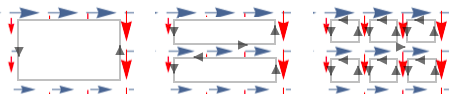
\includegraphics[width=\linewidth]{img/C24p1-21.png}
\end{center}
\end{itemize}
\end{tcolorbox}

\eject


\noindent\textbf{Scalar curl is circulation density} \S 18.4
\begin{tcolorbox}
\begin{itemize}
    \item \textbf{Green's theorem}: Let $R$ be a region in the plane with boundary $C = \partial R$ oriented so that $R$ is on the left as we move along curve $C$.  Then \[\int_R  \frac{\partial Q}{\partial x} - \frac{\partial P}{\partial y}\ dA = \oint_C \mb F \cdot d\mb r.\]
    \item Integrating the scalar curl over a region returns the circulation of the vector field about that region, so the scalar curl is also referred to as the \textbf{circulation density}.
    \item $\partial R$ is the notation for ``the boundary of region R''.
    \item For a simple closed curve $C$ enclosing a region $R$, moving along $C$ in the direction of the orientation, the region $R$ will be on the left when $C$ is oriented counter-clockwise (positive orientation).
    \item On a region $R$ where Green's theorem applies (so on a region where $\mb F$, and the scalar curl of $\mb F$, are defined everywhere), if $\mb F = P\mb i + Q\mb j$ is irrotational, then $\displaystyle\oint_{\partial R}\vec F\cdot d\vec r = 0$.
\end{itemize}
 

\end{tcolorbox}

\noindent\textbf{Example (using Green's theorem)}.

Use Green's thereom to find $\displaystyle\oint_C (x^2+y^2)dx + (x^2+y^2)dy$ where $C$ is the curve defined by $y = x$, $y = x^2$, $0\leq x\leq 1$ with counterclockwise orientation.

The vector field is defined everywhere in the $xy$-plane, and so is the scalar curl.

\begin{enumerate}
    \item Is $C$ a closed curve?  (It is).
    \item Identify $\vec F$.
    \vspace{0.5in}
    
    \item Compute the scalar curl.
    \vspace{1in}
    
    \item Sketch the region $R$.
    
    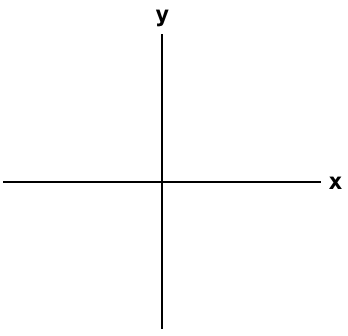
\includegraphics[height=2in]{img/C02axes-2.png}
    
    \item Set up the integral $\int_R Q_x - P_y \ dA$.
    \vspace{1in}
    
    \item Integrate to compute $\oint_{\partial R} (x^2+y^2)dx + (x^2+y^2)dy$.
    \vspace{1.5in}
    
    \item Check whether the orientation of $\partial R$ is the same as the orientation of $C$ (or is opposite).
\end{enumerate}

\vspace{0.2cm}
\hrule
\vspace{0.2cm}

\end{document}